Whereas secondary structures are mainly determined by local interactions, 
so are tertiary structures in addition influenced by distant interactions. 
Hydrophobic interactions are the main driving force in determining the tertiary structure, 
but hydrogen bonds, 
disulfide bonds 
and ionic bonds 
play an important role as well 
(\cite{madigan2015}). 
It is thermodynamically more stable to cluster hydrophobic groups together than expose them to the aqueous environment. 
Therefore, a protein folds in such a way that nonpolar sidechains are buried inside the core 
and polar sidechains reside on the surface.
Multiple macromolecules can form a complex with the tertiary structure, this is called the quaternary structure.
Proteins are versatile in that the tendency to form specific local and distant interactions,
which secondary structures will be formed, 
and even the final fold, 
are all encoded within the primary structure (Fig. \ref{fig:topology})
(\cite{berg2015}).


~\begin{figure}[h!]
	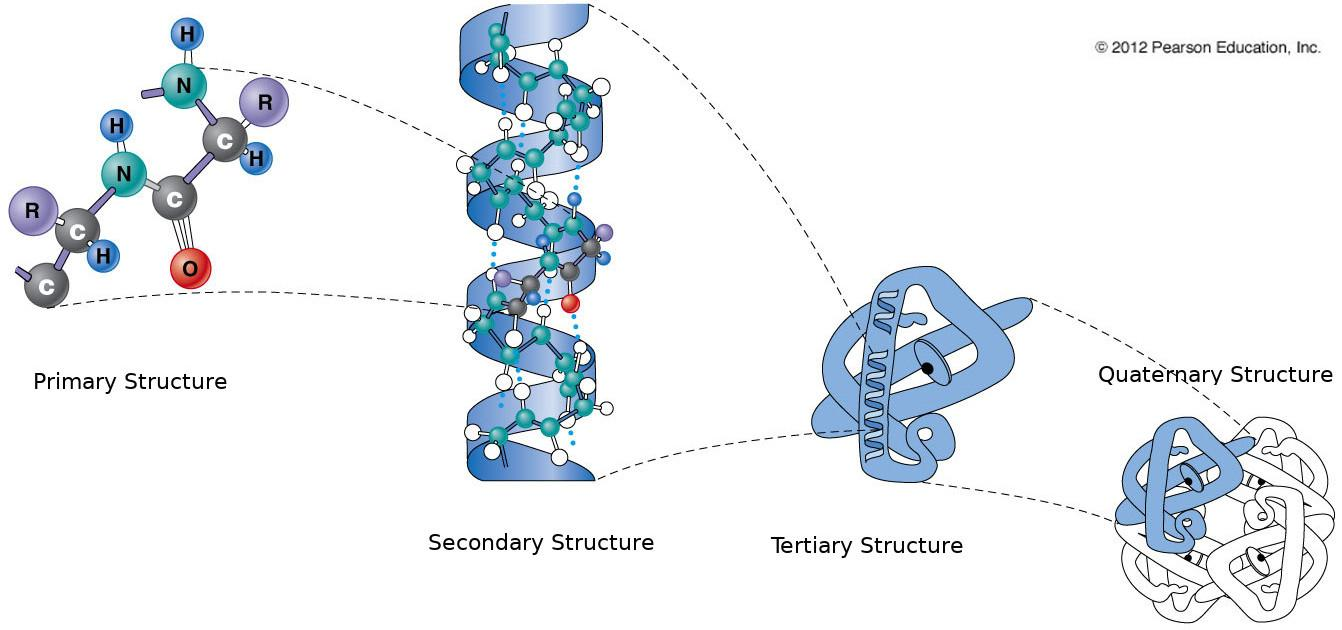
\includegraphics[width=\linewidth]{./literature_review/proteins/tertiary_quaternary/img/topology.jpg}
	\caption{\textbf{Different levels of protein topology.}}
	\label{fig:topology}
~\end{figure}
